\chapter{結果}\label{chap_result}
%loss,accのグラフは全て.
%前処理を行った場合は,その画像の一例も載せる
%モデルの画像(appendixの方がいいかもしれないです)
%各sectionで異なる場合は各sectionで載せましょう
%なるべくpdfで保存しましょう

\section{古典的な画像処理手法による識別精度評価}
%楕円検出の塗った画像
%loss,accのグラフ


\section{教師あり学習による識別精度評価}
% 実際のラベルの画像
% loss, accグラフ



\section{教師なし学習による識別精度評価}
% 潜在空間の分布
% 写真での分布
% loss, accグラフ
\subsection{VAE}
擬似HE染色した画像と,元のカラー画像のそれぞれにVAEを行って潜在変数を2次元プロットした結果.
\begin{figure}
	\centering
\subfigure[]{
	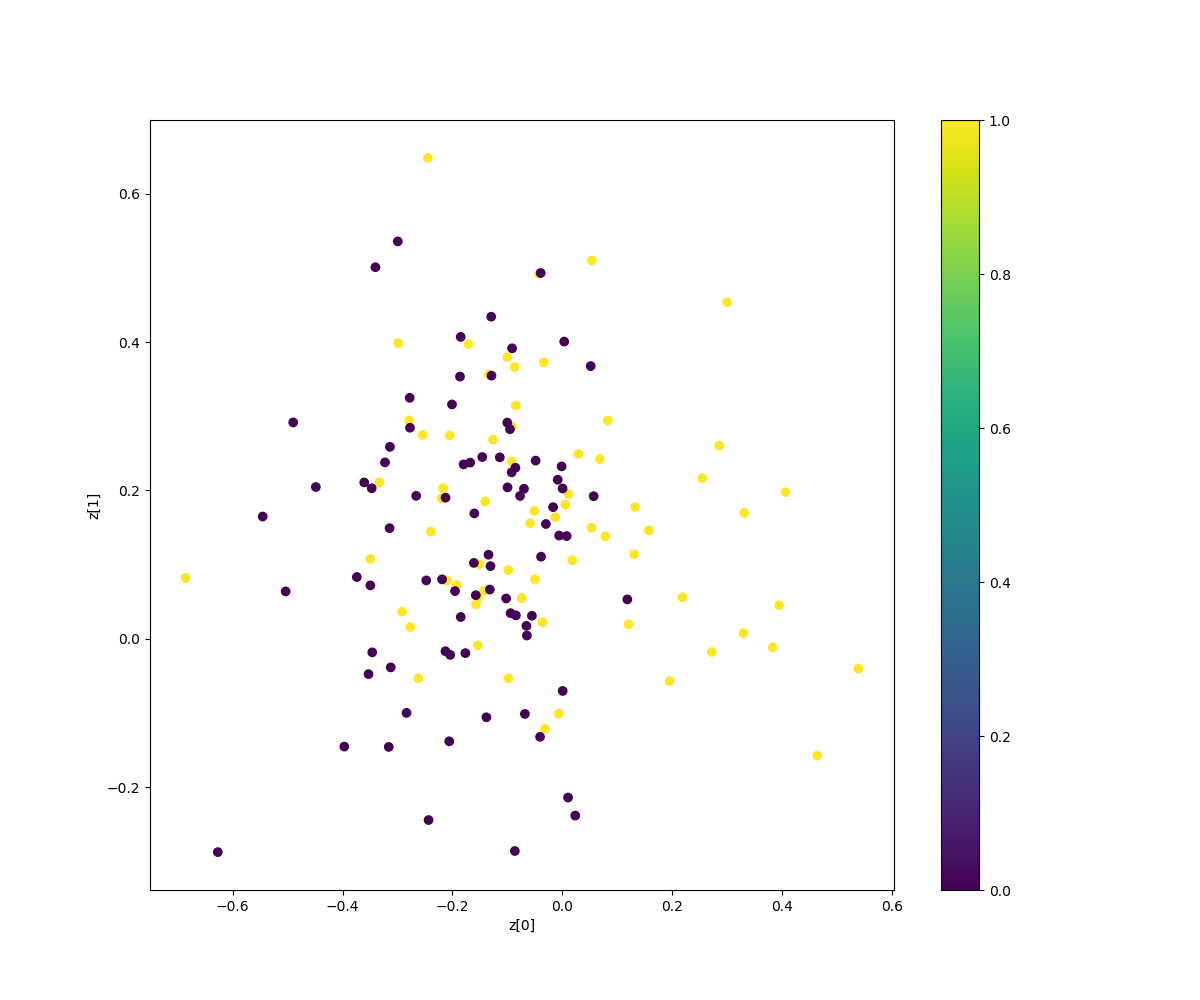
\includegraphics[clip, width=0.4\linewidth]{fig/variational_auto_encoder/vae_colon_epoch_100_c13_he}
}
\subfigure[]{
	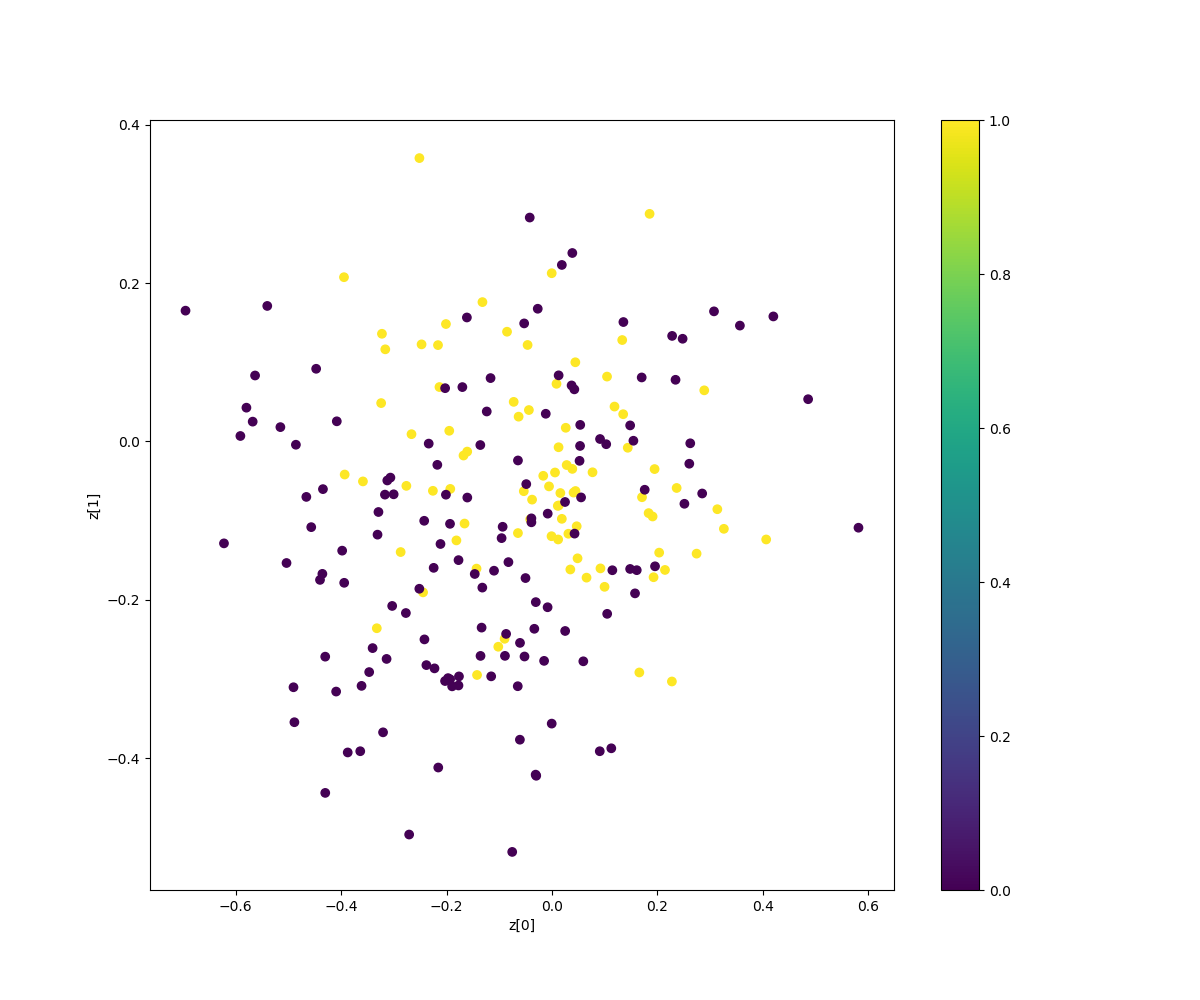
\includegraphics[clip, width=0.4\linewidth]{fig/variational_auto_encoder/vae_colon_epoch_299_c13_rgb}
}

\subfigure[]{
	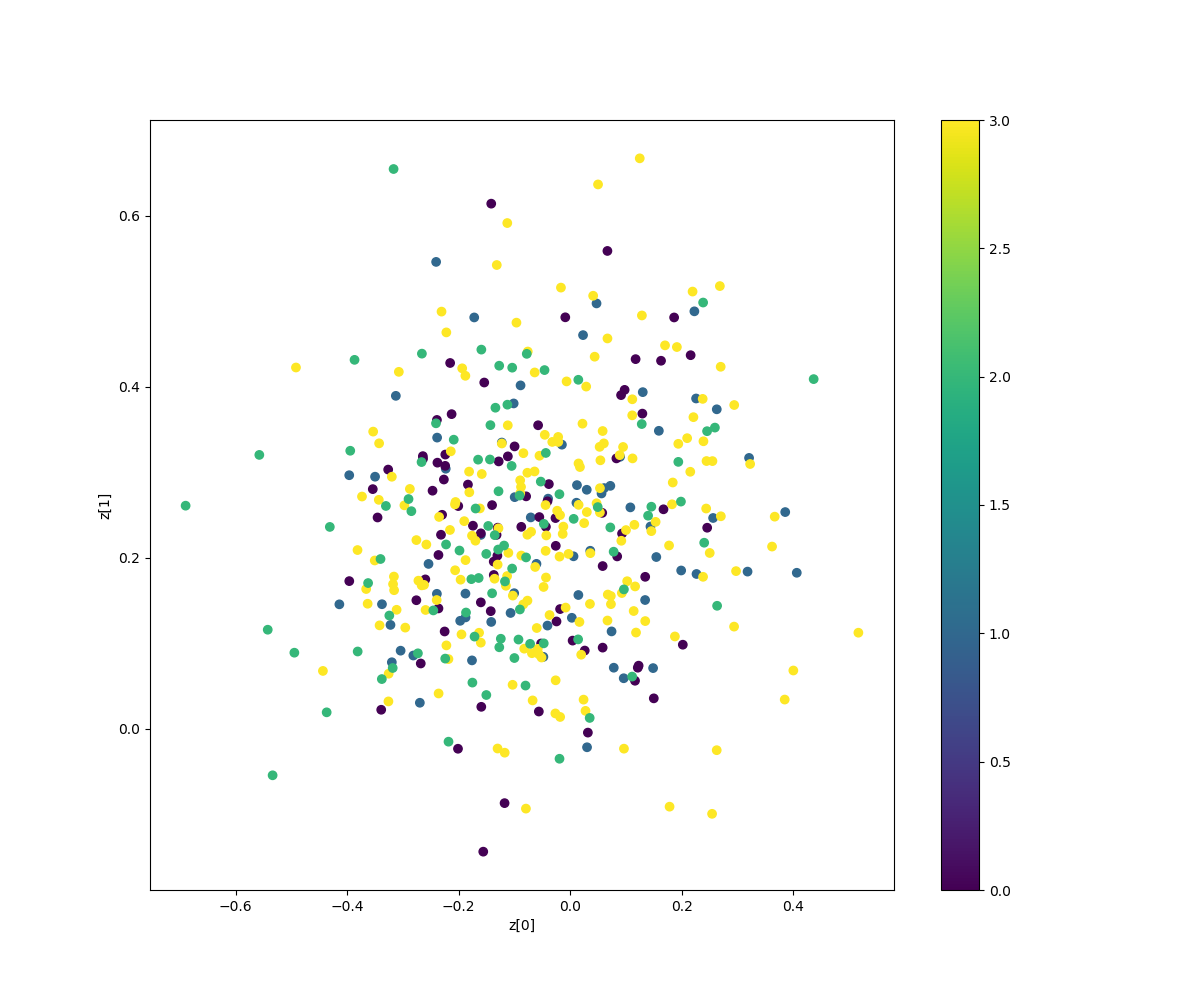
\includegraphics[clip, width=0.4\linewidth]{fig/variational_auto_encoder/vae_colon_epoch_100_he_mix}
}
\subfigure[]{
	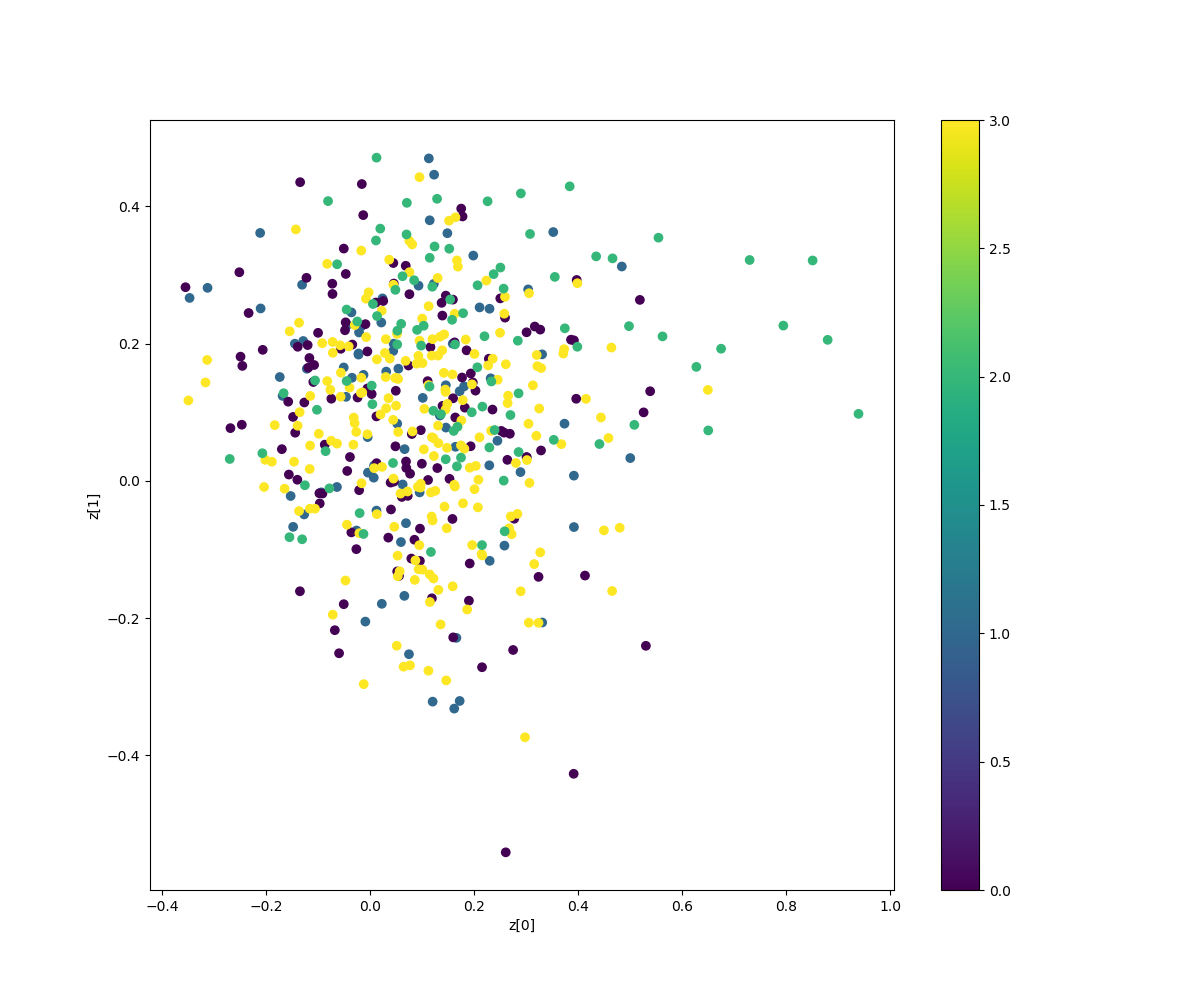
\includegraphics[clip, width=0.4\linewidth]{fig/variational_auto_encoder/vae_colon_epoch_100_rgb_mix}
}
\caption{}
\label{fig:}
\end{figure}

\subsection{GAN}

\begin{figure}
	\centering
\subfigure[epoch=0]{
    
\includegraphics[clip, width=0.4\linewidth]{fig/generative_adversarial_nets/0000_0000}
}
\subfigure[]{
	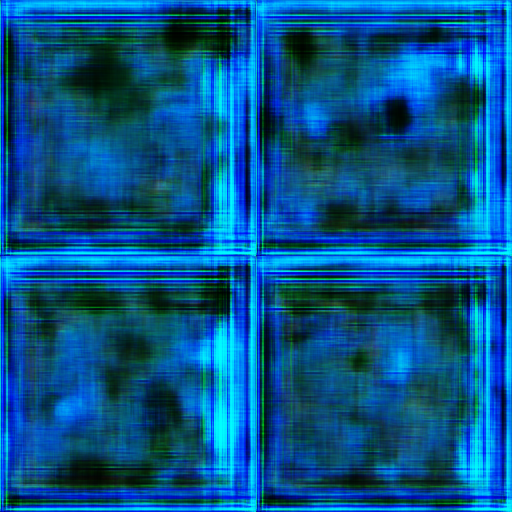
\includegraphics[clip, width=0.4\linewidth]{fig/generative_adversarial_nets/0079_0000}
}
\subfigure[]{
	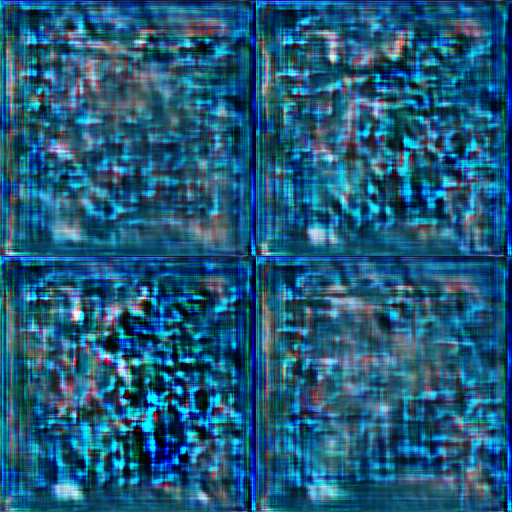
\includegraphics[clip, width=0.4\linewidth]{fig/generative_adversarial_nets/0641_0000}
}
\subfigure[]{
	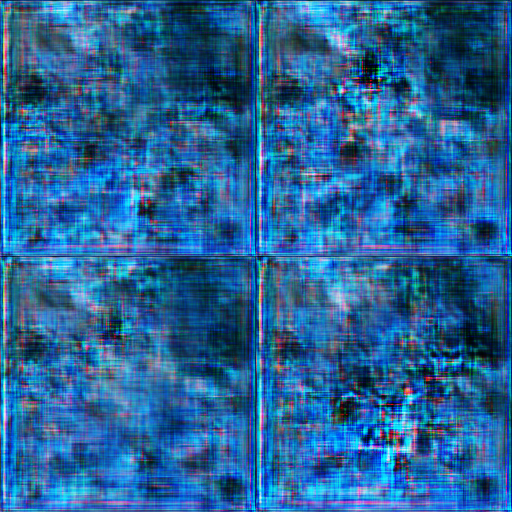
\includegraphics[clip, width=0.4\linewidth]{fig/generative_adversarial_nets/0969_0000}
}
\subfigure[]{
	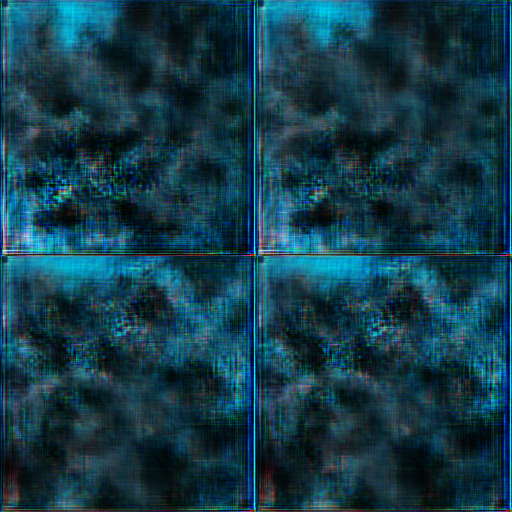
\includegraphics[clip, width=0.4\linewidth]{fig/generative_adversarial_nets/1213_0000}
}
\subfigure[epoch=0]{
	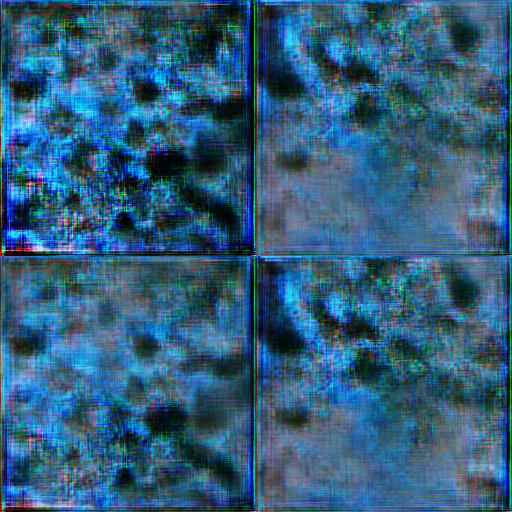
\includegraphics[clip, width=0.4\linewidth]{fig/generative_adversarial_nets/1619_0000}
}
\subfigure[]{
	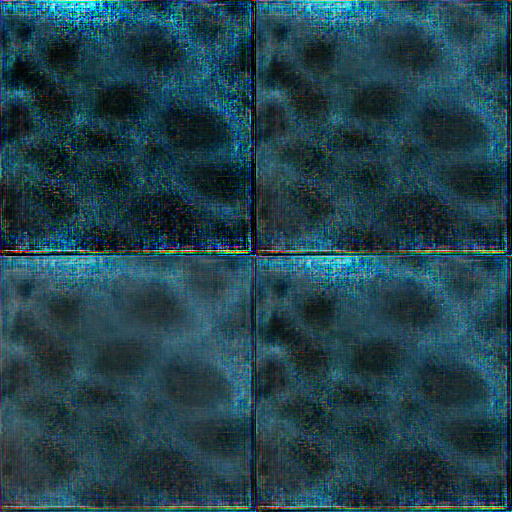
\includegraphics[clip, width=0.4\linewidth]{fig/generative_adversarial_nets/2004_0000}
}
\subfigure[]{
	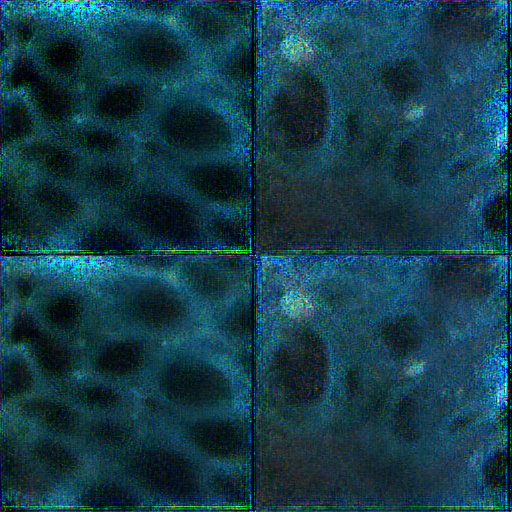
\includegraphics[clip, width=0.4\linewidth]{fig/generative_adversarial_nets/3208_0000}
}
\caption{}
\label{fig:}
\end{figure}


\section{半教師あり学習による識別精度評価}

%lossとaccグラフ
% 教師ありと半教師ありを同じグラフにaccをプロット